\section{The Framework}

The Semantic Web defines a set of technologies which are a standard on how to
describe, manipulate and query Semantic data to have in the end a solid base of
machine-readable knowledge. The Semantic Web presents a layer hierarchy
(Figure~\ref{fig:sw-stack}), where each layer has its own purpose. A layer of
this Semantic Web Stack uses the information provided by layers below. This
shows how Semantic Web is made possible and how it is not a replacement of the
current Web but an extension.

\begin{figure}
\centering
\resizebox{0.5\linewidth}{!}{%
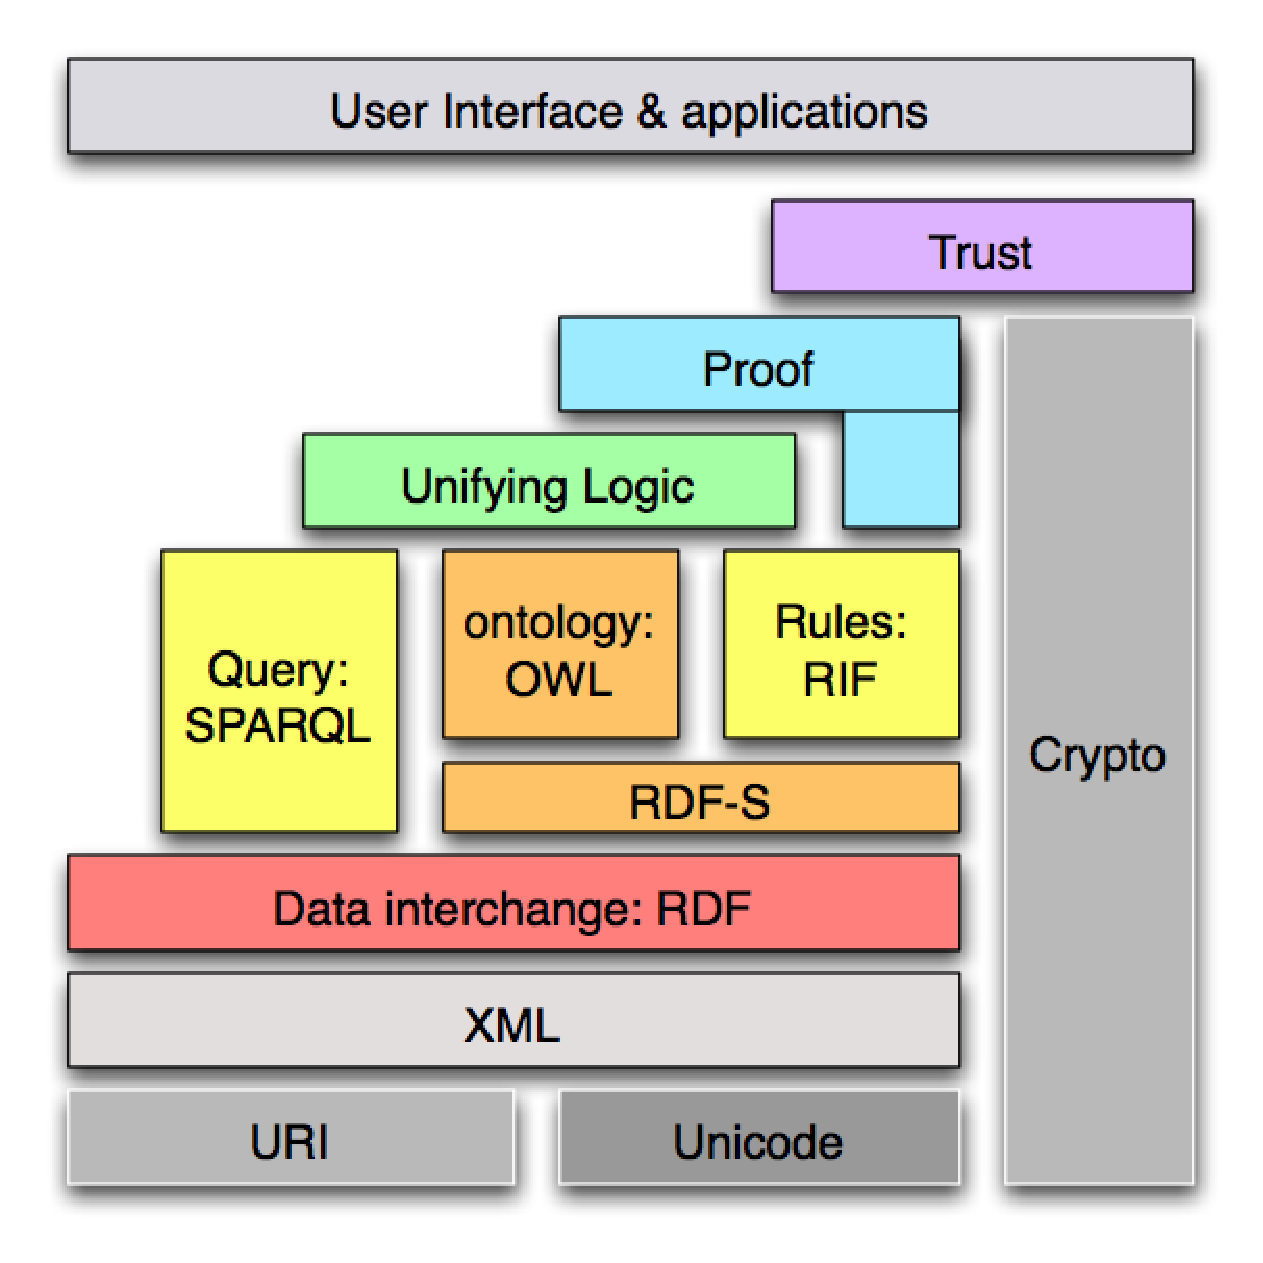
\includegraphics[scale=1]{pics/SemWebStack}
}%
\caption{The Semantic Web Stack. It presents each layer of the Semantic Web,
where each have a defined a purpose and that make the Semantic extension of the
Web as we know it possible.}
\label{fig:sw-stack}
\end{figure}

\begin{description}
\item[Uniform Resource Identifier (URI)] provides means for uniquely
identifying semantic web resources.
\item[Unicode\footnote{\url{http://www.unicode.org/standard/versions/}}] 
serves to represent and manipulate text in many languages. Semantic Web should
also help to bridge documents in different human languages, so it should be
able to represent them.
\item[XML] extensible Markup Language (XML) is the standard syntax that
enables creation of documents composed of structured data. Semantic web gives
meaning (semantics) to structured data. 
\item[Resource Description Framework (RDF)] is the standardized representation
of meta-data.
\item[RDF Schema (RDFS)] provides basic vocabulary for RDF.
\item[Web Ontology Language (OWL)] extends RDFS and allows a more complex
representation of resources (i.e., ontology). It gives then the possibility of
more advanced reasoning over data.
\item[SPARQL] is a RDF query language. It can be used to query any RDF-based
data and provide information to Semantic Web applications.
\item[Logic-Proof] a reasoning layer that infers new knowledge from the data.
\item[Trust] prove the trustfulness of the data thanks to cryptographic
techniques.
\item[User Interface] is the final layer that will enable humans to use
semantic web applications.
\end{description}

URI is a string that is used to identify resources over the Internet. It is
often used by markup languages to specify external documents or a specific
section of that document. For instance \emph{\url{http://di2.deri.ie/}} is an
URI that describes the Data Intensive Infrastructure unit.

An ontology in Information Science is a formal representation of knowledge as a
set of concepts within a domain, and the relationships between those concepts.
It is used to reason about the entities within that domain, and may be used to
describe the domain. For example we can have a simple ontology describing
animals like rats and cats are mammals; a mammal is an animal. Such an ontology
can be used when searching for terms in different domains.

\section{RDF: Resource Description Framework}

RDF is a framework that allows data on the web to be shared and reused across
applications. It provides features that facilitate data to be interchange
between datasets, even if they have different ontology.
RDF is used to describes things in the Internet, and the relations between
things. It extends the linking structure of the Web to use URIs to name the
relationship between concepts or objects as well as the two ends of the link.
This linking structure of the Web forms a directed, labeled graph called
\emph{RDF graph}, where the edges represent the relationship between two
objects, the graph nodes.

\subsection{RDF Model}

RDF is a standard
model\footnote{\url{http://www.w3.org/TR/2004/REC-rdf-concepts-20040210/\#section-Concepts}}
for data interchange on the Web. Two connected nodes and the named relation
form a \emph{triple}. The set of triples form the RDF graph. The three parts
that compose a triple are:
\begin{enumerate}
  \item a \emph{subject}: the resource that this triple describes.
  \item an \emph{object}: the resource that the subject is related to.
  \item a \emph{predicate}: the description of the link between the subject and
  the object.
\end{enumerate}
The Figure~\ref{fig:rdf-triple} depicts a triple as a node-arc-node
link. The direction of the arc is significant: it always points toward the
object. The nodes of an RDF graph are its subjects and objects. The meaning
given to a RDF graph is the conjunction of all its triples.

A RDF graph defines three types of nodes:
\begin{description}
\item[Literal] a literal is a simple string, used to describe dates, titles or
any text in natural language. A literal may be \emph{plain} or \emph{typed}:
	\begin{itemize}
	  \item A plain literal is a string combined with an optional language tag.
	  \item A typed literal is a string combined with a datatype URI.
	\end{itemize}
\item[URI reference (URIref)] a URIref is a Unicode string used in a RDF graph
to represent URIs, and it can have an optional fragment identifier which is
indicated by the character ``\#''. For example the URI reference
\url{http://www.w3.org/2000/01/rdf-schema#comment} shows the URI before \#, and
the fragment ``comment'' that indicates which identifier to use within the URI.
This particular fragment ``comment'' is used to describe the subject resource.
\item[Blank Node] a blank node refers to resources that are not identified.
\end{description}
In a triple, the subject can be either a URIref or a blank node. The predicate
must be a URIref, while the object can be either one of the three node types.

The URI tends to be very long, which becomes inconvenient when using frequently
a same URIref. QName is a name space used as an abbreviation of a URIref. Its
syntax is \emph{URI:fragment}. For example the fragment ``comment'' within the
URI \url{http://www.w3.org/2000/01/rdf-schema#} can be shortened to
\emph{rdfs:comment}, where rdfs is mapped to the URI.

In the drawing convention of a RDF graph, URIrefs and blank nodes are drawn with an
ellipse, and literals with a rectangle. The Figure~\ref{fig:rdf-graph} depicts
a RDF graph describing the work ``The Lord of the Rings'' written by J.R.R
Tolkien. In this graph, the QNames ``dbpprop'' and ``dbpedia-owl'' map
respectively to \emph{\url{http://dbpedia.org/property/}} and
\emph{\url{http://dbpedia.org/ontology/}}. This graph provides three different
triples describing the sequel. The RDF graph gives the meaning that the
resource \url{http://dbpedia.org/page/The_Lord_of_the_Rings} has for author
J.R.R Tolkien, that it was released in the years 1954-55 and that a portion of
the English abstract is ``The Lord of the Rings is an epic\ldots''. We also
know that an unknown resource preceding ``The Lord of the Rings" novel was also
written by Tolkien.

\begin{figure}
\resizebox{\linewidth}{!}{%
\subfloat[A triple]{%
\centering
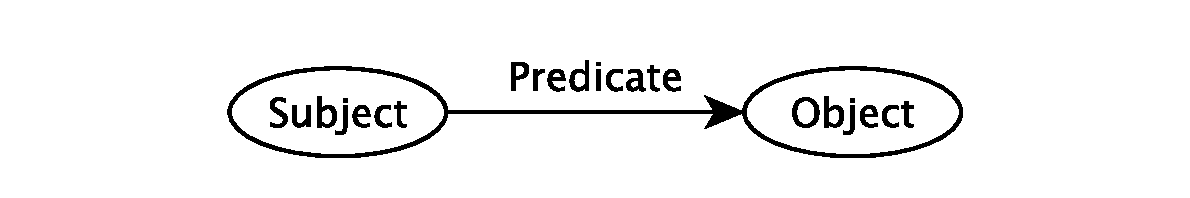
\includegraphics[scale=0.4]{pics/rdf-triple}
\label{fig:rdf-triple}
}\quad
\subfloat[A RDF graph describing the work ``The Lord of the Ring'' by J.R.R
Tolkien, using several QNames.]{%
\centering
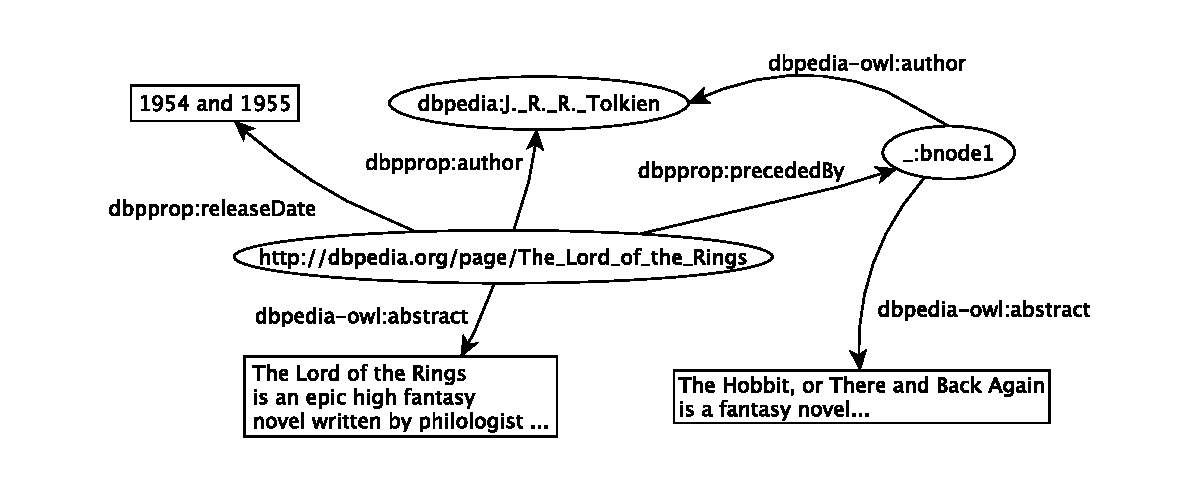
\includegraphics[scale=0.5]{pics/rdf-graph}
\label{fig:rdf-graph}
}}%
\caption{The RDF model used to represent knowledge.}
\end{figure}

\subsection{RDF Serialization}

Many serialization format for RDF have been developed, such as
RDFa\footnote{\url{http://www.w3.org/TR/xhtml-rdfa-primer/}} which is used to
embed RDF triples within XML documents. However during my internship only the
serialization format
\emph{N-Triple}\footnote{\url{http://www.w3.org/TR/rdf-testcases/\#ntriples}}
has been actively used, and so it will be the only one described here. Using
the N-Triple format, the triples within a RDF graph can be serialized with a
line-based plain text format. It is a format recommended to interchange data
between different applications.

This serialization uses an Extended Backus-Naur Form grammar, where each triple
is written into a line, ending with a point. The format is {\bfseries
\emph{Subject Predicate Object .}}\hs.
A URIref is written enclosed between the characters \emph{'$<$' '$>$'}. The
literals are written between double quotes, followed by an optional language
tag \emph{@language} for plain literals (e.g. ``bird"@en), and by
\emph{'\^{}\^{}'URIref} for typed literal (e.g.
``abc"\^{}\^{}$<$\url{http://example.org/datatype1}$>$, where abc is of type
datatype1). A blank node is represented by \emph{'\_':name}, where name is an
internal identifier which allows to have several blank nodes within a RDF
graph. The RDF graph in the Figure~\ref{fig:rdf-graph} can be serialized in
N-Triples format as in Table~\ref{tab:TL-ntriples} where \emph{TLR} refers to
the URI \url{http://dbpedia.org/page/The_Lord_of_the_Rings}.

\begin{table}
\centering
\resizebox{0.9\linewidth}{!}{%
\begin{tabular}{lclclcl}
$<$TLR$>$&\phantom{a}&$<$dbpprop:author$>$&\phantom{a}&$<$dbpedia:J.\_R.\_R.\_Tolkien$>$
&\phantom{a}&.\\
$<$TLR$>$&\phantom{a}&$<$dbpprop:releaseDate$>$&\phantom{a}&``1954 and
1955''&\phantom{a}&.\\
$<$TLR$>$&\phantom{a}&$<$dbpedia-owl:abstract$>$&\phantom{a}&``The Lord of
the Rings is an epic\ldots''&\phantom{a}&.\\
$<$TLR$>$&\phantom{a}&$<$dbpprop:precededBy$>$&\phantom{a}&$\_:bnode1$&\phantom{a}&.\\
$\_:bnode1$&\phantom{a}&$<$dbpedia-owl:author$>$&\phantom{a}&$<$dbpedia:J.\_R.\_R.\_Tolkien$>$&\phantom{a}&.\\
$\_:bnode1$&\phantom{a}&$<$dbpedia-owl:abstract$>$&\phantom{a}&''The Hobbit, or
There and Back Again is a fantasy novel\ldots''&\phantom{a}&.\\
\end{tabular}
}%
\caption{N-Triple representation of the RDF graph in
Figure~\ref{fig:rdf-graph}.}
\label{tab:TL-ntriples}
\end{table}

\subsection{SPARQL}

The RDF model introduce a mean to represent data and any type of data can,
at least to some degree, be represented in this model. SPARQL\footnote{SPARQL:
\url{http://www.w3.org/TR/rdf-sparql-query/}} is a standardized query language
for RDF. Designed so that queries can be expressed across diverse data, SPARQL
is able to express not only conjunction and disjunction of RDF graphs but also
complex queries, e.g. by using supplementary binary operators such as
arithmetic operators and comparisons in various filters.

A SPARQL query contains a set of \emph{triple patterns} that matches a
sub-graph of RDF graphs. Triple patterns are expressed in the same way as RDF
triples, i.e., subject, predicate, object, the difference being that any part of
that triple can be a variable. Typical SPARQL queries are graph patterns
combining SQL-like logical conditions over RDF statements with
regular-expression patterns. The result of a query is a set of sub-graphs
matching precisely the graph pattern defined in the query. For instance, the
SPARQL query
\begin{quote}
\begin{flushleft}
PREFIX dbpprop:    $<$http://dbpedia.org/property/$>$\\
SELECT ?abstract\\
WHERE\\
\{\\
\begin{quote}
$<$TLR$> \; <$dbpprop:author$> \;$ ?abstract $\;$ . 
\end{quote}
\}
\end{flushleft}
\end{quote}
has a single triple pattern that matches the first row of the triples in the
Table~\ref{tab:TL-ntriples}. The first line shows the QName used in the query.

% \subsection{Reasoning}
% 
% Reasoning is the cognitive process to look for conclusions and beliefs.
% Reasoning allows to create links between two objects that are somehow related
% but only implicity, granting thus the machine to enlarge its searching scope.
% For example, we know that a monkey is a mamal and that mammals are an animal
% species, but how can a machine deduces that a monkey is also an animal. Through
% reasoning over RDF graphs, it is possible to ``create'' more knowledge,
% \emph{implicit} knowledge, from the explicit relations already existing. For
% example, the RDFS schema possesses inheritance reasoning capabilities
% through the property \emph{subClassOf} such as
% \begin{quotation}
% (rdf:type Morris Cat)
% 
% (rdfs:subClassOf Cat Mammal),
% \end{quotation}
% which implies that Morris is also a sub-class of mammal.
